% This contents of this file will be inserted into the _Solutions version of the
% output tex document.  Here's an example:

% If assignment with subquestion (1.a) requires a written response, you will
% find the following flag within this document: <SCPD_SUBMISSION_TAG>_1a
% In this example, you would insert the LaTeX for your solution to (1.a) between
% the <SCPD_SUBMISSION_TAG>_1a flags.  If you also constrain your answer between the
% START_CODE_HERE and END_CODE_HERE flags, your LaTeX will be styled as a
% solution within the final document.

% Please do not use the '<SCPD_SUBMISSION_TAG>' character anywhere within your code.  As expected,
% that will confuse the regular expressions we use to identify your solution.

\def\assignmentnum{1 }
\def\assignmenttitle{XCS234 Assignment \assignmentnum}
\input{macros}
\begin{document}
\pagestyle{myheadings} \markboth{}{\assignmenttitle}

% <SCPD_SUBMISSION_TAG>_entire_submission

This handout includes space for every question that requires a written response.
Please feel free to use it to handwrite your solutions (legibly, please).  If
you choose to typeset your solutions, the |README.md| for this assignment includes
instructions to regenerate this handout with your typeset \LaTeX{} solutions.
\ruleskip

\LARGE
1.b
\normalsize
% <SCPD_SUBMISSION_TAG>_1b
\begin{answer}
  % ### START CODE HERE ###
  \textbf{Behavior Cloning Results}

  Both environments were tested with identical hyperparameters for fair comparison:
  \begin{itemize}
    \item Network: 2 hidden layers, 64 units each
    \item Training steps: 1000 gradient updates
    \item Learning rate: 5e-3
    \item Eval batch size: 5000 (for multiple rollouts)
  \end{itemize}

  \begin{center}
  \begin{tabular}{|l|c|c|c|c|}
    \hline
    \textbf{Environment} & \textbf{Expert Return} & \textbf{BC Mean} & \textbf{BC Std} & \textbf{\% of Expert} \\
    \hline
    Ant-v4 (working) & 4713.65 & 1551.48 & 993.03 & 32.9\% \\
    \hline
    Walker2d-v4 (not working) & 5566.85 & 295.01 & 341.21 & 5.3\% \\
    \hline
  \end{tabular}
  \end{center}

  \textbf{Analysis:} BC achieves $>$30\% on Ant-v4 but fails on Walker2d-v4 (only 5.3\%).
  Walker2d requires precise balance and timing that BC struggles to learn from static
  demonstrations. The high standard deviation in Walker2d (341.21) indicates inconsistent
  behavior, with episodes often terminating early (avg episode length: 126 vs 1000 for expert).
  % ### END CODE HERE ###
\end{answer}
% <SCPD_SUBMISSION_TAG>_1b
\clearpage

\LARGE
1.c
\normalsize

% <SCPD_SUBMISSION_TAG>_1c
\begin{answer}
  % ### START CODE HERE ###
  \textbf{Hyperparameter:} \texttt{num\_agent\_train\_steps\_per\_iter}

  \textbf{Rationale:} This hyperparameter controls how many gradient updates the policy
  network receives during training. It directly affects the underfitting/overfitting
  trade-off: too few steps means the policy hasn't learned the expert behavior, while
  too many steps could lead to overfitting on the limited expert data.

  \textbf{Experiment:} Tested on Ant-v4 with values: 100, 500, 1000, 1500, 2000, 3000, 4000, 5000, 6000.

  \begin{center}
  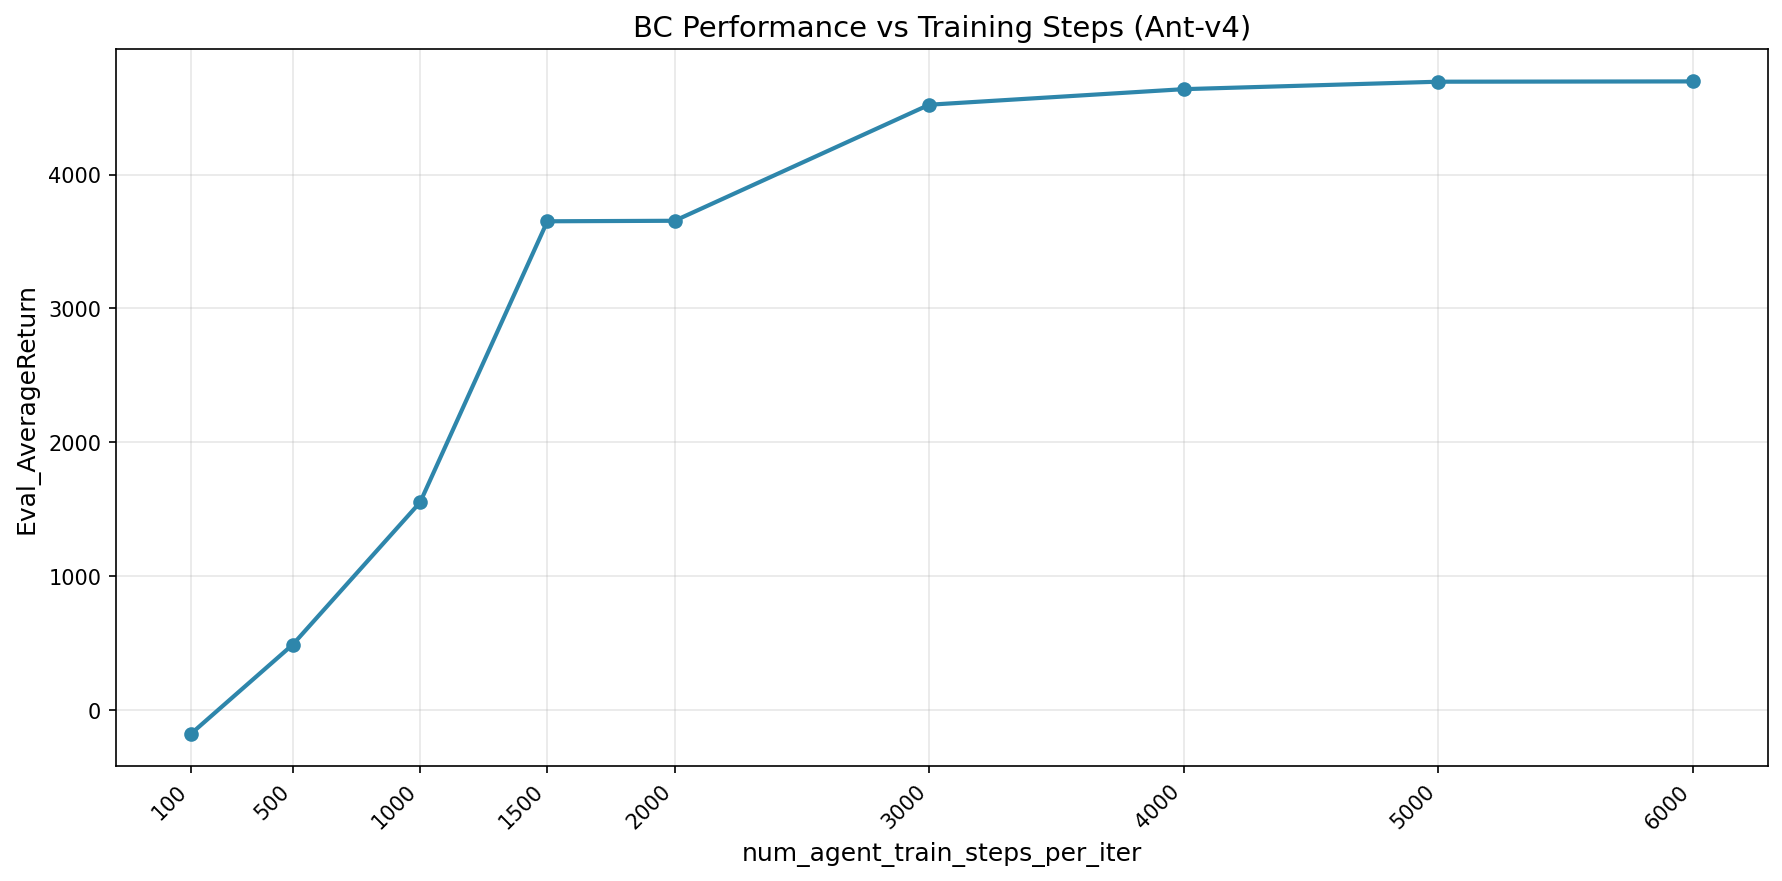
\includegraphics[width=0.85\textwidth]{bc_train_steps_experiment.png}
  \end{center}

  \textbf{Results:} Performance increases rapidly from 100 to 3000 steps, then plateaus
  near expert level ($\sim$4700). At 100 steps, the policy is severely underfit (negative return).
  No overfitting was observed up to 6000 steps, suggesting the expert dataset is sufficient
  for this task.
  % ### END CODE HERE ###
\end{answer}
% <SCPD_SUBMISSION_TAG>_1c
\clearpage


\LARGE
2.b
\normalsize

% <SCPD_SUBMISSION_TAG>_2b
\begin{answer}
  % ### START CODE HERE ###
  % ### END CODE HERE ###
\end{answer}
% <SCPD_SUBMISSION_TAG>_2b
\clearpage

% <SCPD_SUBMISSION_TAG>_entire_submission

\end{document}
